\documentclass[11pt, hidelinks, a4paper]{report}

\usepackage{fancyhdr}							% Nagłówek
\usepackage[margin=1in]{geometry}				% Margines
\usepackage{wrapfig}
\usepackage{hyperref}							% Linki
\usepackage{fix-cm}
\usepackage{tikz}
\usepackage[document]{ragged2e}
\usepackage{graphicx}							% Grafiki
\usepackage[polish]{babel}						% Język polski
\usepackage[]{float}							% Umiesczanie grafik i tabel w dowolnych miejscach
\usepackage{pdfpages}							% Wklejanie stron pdf
\usepackage{tabularx}							% Tabele
\usepackage{array}
\usepackage{caption}							% Podpisy
\usepackage[T1]{fontenc}							% Czcionki
%\usepackage{subfig}								% Rysunki dzielone
\usepackage{subcaption}							% Podpisy mniejszych grafik
\usepackage{gensymb}							% Symbole
\usepackage{listings}							% Wklejanie kodu	
\usepackage[justification=centering]{caption}	% Centrowanie podpisów
\usepackage[default]{lato} % Czcionka
\usepackage{listings}
\usepackage{lastpage}
\usepackage{titlesec}
\usepackage[none]{hyphenat}
\usepackage{amsmath}
%\usepackage[table]{xcolor}
\usepackage{colortbl}
\usepackage{fmtcount}
\usepackage{xstring}
%----------------------------------------------------------------------------------------------------------------------------
% Definicje kolorów
\definecolor{tableheader}{HTML}{a6a6a6}
%----------------------------------------------------------------------------------------------------------------------------
% Ustawienia wklejanie kodu
\lstset{frame=tb,
	language=C,
	aboveskip=3mm,
	belowskip=3mm,
	showstringspaces=false,
	columns=flexible,
	basicstyle={\small\ttfamily},
	numbers=none,
	numberstyle=\tiny\color{gray},
	keywordstyle=\color{blue},
	commentstyle=\color{dkgreen},
	stringstyle=\color{mauve},
	breaklines=true,
	breakatwhitespace=true,
	tabsize=3
}
%----------------------------------------------------------------------------------------------------------------------------
% Polskie znaki w kodzie
\lstset{
	literate={ą}{{\k a}}1
	{Ą}{{\k A}}1
	{ż}{{\. z}}1
	{Ż}{{\. Z}}1
	{ź}{{\' z}}1
	{Ź}{{\' Z}}1
	{ć}{{\' c}}1
	{Ć}{{\' C}}1
	{ę}{{\k e}}1
	{Ę}{{\k E}}1
	{ó}{{\' o}}1
	{Ó}{{\' O}}1
	{ń}{{\' n}}1
	{Ń}{{\' N}}1
	{ś}{{\' s}}1
	{Ś}{{\' S}}1
	{ł}{{\l}}1
	{Ł}{{\L}}1
}
%----------------------------------------------------------------------------------------------------------------------------
% Ścieżka do grafik
\graphicspath{{../../img/}}
%----------------------------------------------------------------------------------------------------------------------------
% Definicje
\def\companyname{Koło Naukowe Mikrosystemów ONYKS}
\def\revision{1.0}
\def\docnumber{UGHW1}
\def\lang{PL}
\def\repolink{github.com/knonyks/ATXMEGA256_miniboard}

\def\headerheight{1cm}
%----------------------------------------------------------------------------------------------------------------------------
% Nagłówek
\pagestyle{fancy}
\setlength{\headheight}{\headerheight}
\renewcommand{\headrulewidth}{0pt}

\fancyhf{}
\fancyhead[R]{
	
\includegraphics[height=\headerheight]{logo.png}
}
\fancyhead[L]{\leftmark}
%----------------------------------------------------------------------------------------------------------------------------
% Stopka
\fancyfoot[L]{\docnumber(\lang) \space Rev. \space \revision, \space \today \hfill \thepage \space\space /  \space \pageref{LastPage}}
%----------------------------------------------------------------------------------------------------------------------------
% Redefinicja stylu plain
\fancypagestyle{plain}{
	\fancyhf{}
	\fancyhead[R]{
		
\includegraphics[height=\headerheight]{logo.png}
	}
	\fancyhead[L]{\leftmark}
	\fancyfoot[L]{\docnumber(\lang) \space Rev.\space \revision, \space \today \hfill \thepage \space\space / \space \pageref{LastPage}}
}
%----------------------------------------------------------------------------------------------------------------------------
% Wyłączenie dzielenia wyrazów
\tolerance=1
\emergencystretch=\maxdimen
\hyphenpenalty=1000
\hbadness=1000
%----------------------------------------------------------------------------------------------------------------------------
% Styl rozdziału
\definecolor{onyks-gray}{gray}{0.82}
\definecolor{onyks-red}{HTML}{e50000}
\definecolor{onyks-white}{HTML}{eeeeee}
\titleformat{\chapter}[block]
{\normalfont\Huge\bfseries}
{\colorbox{onyks-gray}{\parbox{\dimexpr0.07\textwidth\relax}{\thechapter}}}
{0.5em}
{\textcolor{onyks-red}{|} \hspace{0.5em}}
%{\thechapter}{0.5em}
%{\textcolor{red}{|} \hspace{0.5em}}
\titlespacing*{\chapter}{0pt}{0pt}{30pt}
%----------------------------------------------------------------------------------------------------------------------------
% Numerowanie stron
\pagenumbering{arabic}
%----------------------------------------------------------------------------------------------------------------------------
% Ustawienia tabel
\renewcommand{\arraystretch}{1.2}
%----------------------------------------------------------------------------------------------------------------------------
\begin{document}
	% Strona tytułowa
	\label{Title}
	\begin{titlepage}
		
		\thispagestyle{empty}
		
		\vspace*{1cm}
		
		\begin{FlushLeft}
			\textbf{\Huge \textcolor{onyks-red}{|}
				ATxmega256 Miniboard\\
				\vspace{10pt}
				\huge Warstwa sprzętowa}\\
			\vspace*{1cm}
			\LARGE Przewodnik użytkownika\\
			\large \docnumber (\lang) \space Rev. \revision\\
			\today
		\end{FlushLeft}
		
		\vfill
		
		\begin{Center}
			
\includegraphics[height=2cm]{logo.png}\\
			\vspace*{1cm}
			\Large \companyname
		\end{Center}
		
		\vspace*{3cm}
		
		
	\end{titlepage}
	\setcounter{page}{2}
	\setcounter{tocdepth}{3}
	\tableofcontents
	
	\justifying
	\sloppy
	
	\chapter{Wstęp}
	Płytka ATxmega256 Miniboard została przygotowana przez KN ONYKS jako projekt edukacyjny mający na celu naukę programowania i projektowania układów z mikrokontroleremi z serii ATxmega256.
	\\
	Materiały dotyczące projektu można znaleźć w oficjalnym repozytorium Github KN ONYKS \textcolor{blue}{\url{\repolink}}.
	\\
	\\
	Ten dokument jest przewodnikiem po części sprzętowej płytki rozwojowej. Instrukcje dotyczące środowiska programowania i debugowania znajdują się w innym dokumencie.
	
	\begin{Center}
		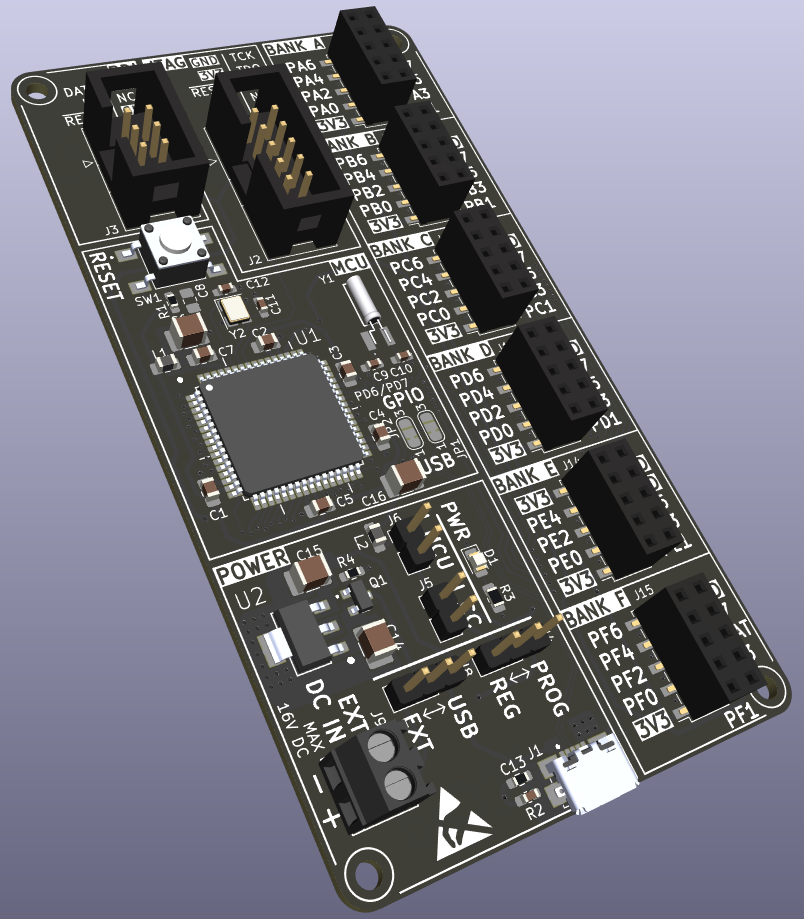
\includegraphics[width=12cm]{ATXMEGA256_Miniboard_top2.png}\\
	\end{Center}

	\chapter{Konfiguracja połączeń}
	Płytka posiada wiele możliwości konfiguracji zasilania oraz interfejsów. W układzie znajduje się tylko absolutne minimum elementów potrzebnych do poprawnego funkcjonowania mikrokontrolera aby użytkownik miał pełną kontrolę na interfejsami, GPIO i zegarami w swoim projekcie.
	
	\section{Opcje zasilania}
	Układ działa poprawnie z nominalnym poziomem napięcia 3,3 V. Istnieje kilka możliwości zasilania płytki:
	\begin{itemize}
		\item Zewnętrzne źródło (EXT)
		\item Micro USB
		\item Zasilanie 3,3 V przez programator
	\end{itemize} 

	\begin{figure}[H]
		\centering
		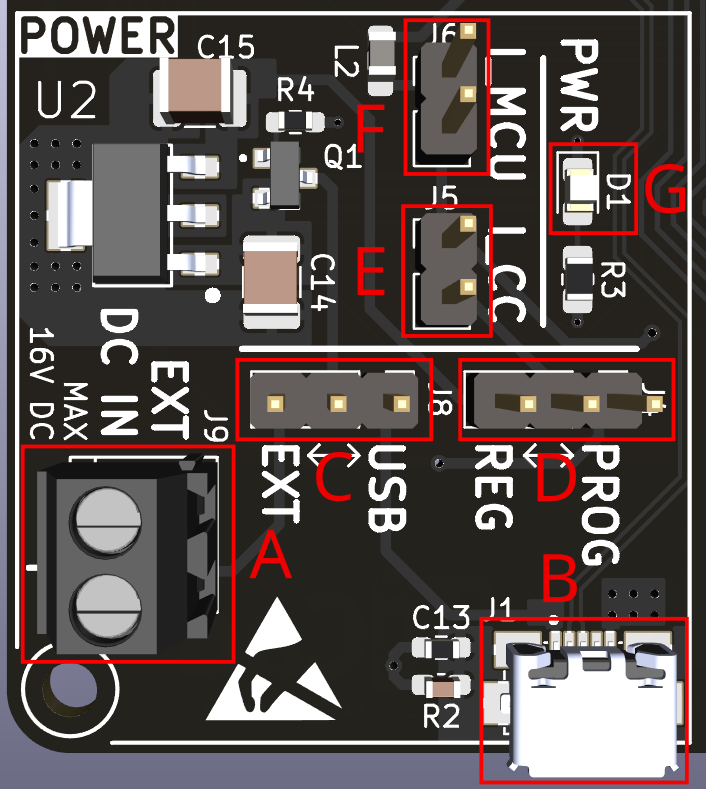
\includegraphics[width=10cm]{power.png}
		\caption{Sekcja zasilania}
	\end{figure}
	\newpage
	Objaśnienia oznaczeń:
	\begin{itemize}
		\item A - złącze śrubowe do podłączenia napięcia zewnętrznego EXT
		\item B - złącze micro USB
		\item C - przełącznik źródła napięcia regulatora 3,3 V:\\ pozycja EXT - napięcie ze złącza śrubowego,\\ pozycja USB - 5 V z micro USB
		\item D - przełącznik źródła 3,3 V:\\ pozycja REG - regulator,\\ pozycja PROG - zasilanie z programatora
		\item E - punkt pomiaru prądu całego układu (zwarty lub podłączony amperomierz)
		\item F - punkt pomiaru prądu samego mikrokontrolera (zwarty lub podłączony amperomierz)
		\item G - LED informujący o podłączonym zasilaniu 3,3 V
	\end{itemize} 

		\subsection{Zewnętrzne źródło (EXT)}
			Zewnętrzne źródło napięcia można podłączyć (zwracając uwagę na polaryzację) przez złącze śrubowe. Minimalne napięcie przy którym układ będzie działać poprawnie to około 4,3 V, a maksymalne 16 V. Ograniczenia wynikają z zastosowanego regulatora napięcia. W przypadku wyższych napięć i dużego poboru prądu można spodziewać się automatycznego wyłączenia regulatora przez osiągnięcie zbyt wysokiej temperatury.
		\subsection{Zasilanie 3,3 V przez programator}
			Układ może być zasilany bezpośrednio z napięcia 3,3 V pochodzącego z programatora podłączonego do odpowiednich złączy programujących. Należy wtedy zewrzeć kontakt środkowy i oznaczony napisem PROG na złączu oznaczonym na rysunku jako D. Taka konfiguracja odłącza wyjście regulatora.
			\\
			Niektóre programatory wymagają podłączenia do napięcia zasilania mikrokontrolera aby dopasować poziomy logiczne ale same nie zasilają układu (przykład: Microchip Pickit Basic w konfiguracji JTAG). Jeżeli układ jest zasilany z innego źródła niż programator to kontakty zasilania 3V3 na złączach programujących będą odłączone (patrz: schemat).
		
	\section{Interfejsy programowania}
		Mikrokontrolery z rodziny ATxmega256 posiadają 2 interfejsy programowania i debugowania:
		\begin{itemize}
			\item PDI (Program and Debug Interface) - własny interfejs Microchip
			\item JTAG (Joined Test and Action Group)
		\end{itemize}
		Interfejs PDI jest zawsze dostępny przez dedykowane nóżki. Interfejs JTAG jest fabrycznie włączony i dostępny przez część pinów GPIO (patrz: schemat). Za pomocą bitów konfiguracyjnych (Fuse Bits) istnieje możliwość jego wyłączenia, a także konfiguracji ID.
		\\
		\\
		\textbf{Należy uważać na GPIO opisane na schemacie, które są współdzielone z JTAG. Nieodpowiednie podłączenie może doprowadzić do uszkodzenia interfejsu lub programatora.} 
		
		\begin{figure}[H]
			\centering
			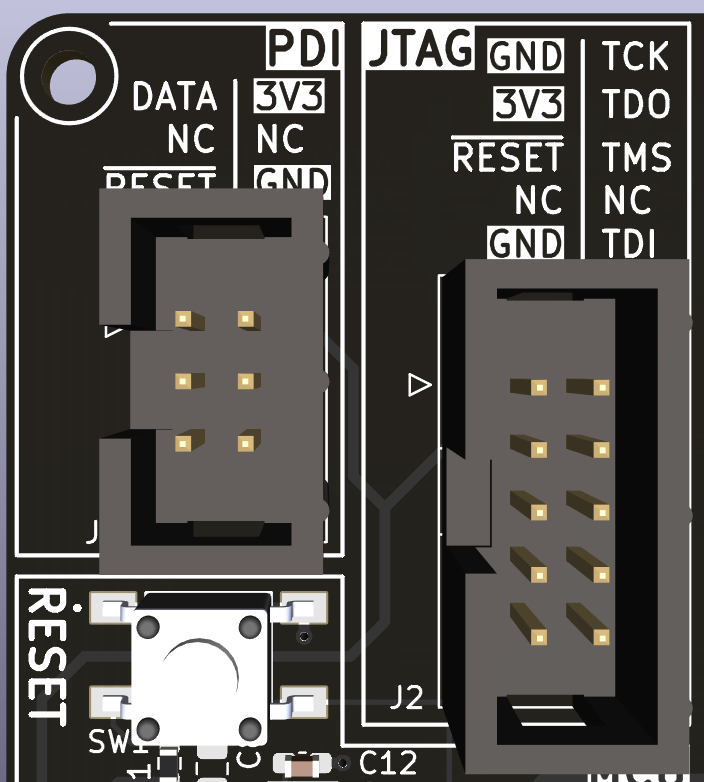
\includegraphics[width=10cm]{programming.png}
			\caption{Sekcja programowania}
		\end{figure}
	
	\section{Zegary}
		Mikrokotrolery z rodziny ATxmega256 posiadają wiele opcji ustawień zegara. Na płytce znajduje się kryształ 16 MHz oznaczony na rysunku \ref{mcu} symbolem I. Dodatkowo podłączony jest też kryształ RTC 32,768 kHz oznaczony symbolem J. W przypadku potrzeby ręcznego resetu mikrokotrolera, znajduje się przy nim przycisk RESET oznaczony symbolem H.
		\begin{figure}[H]
			\centering
			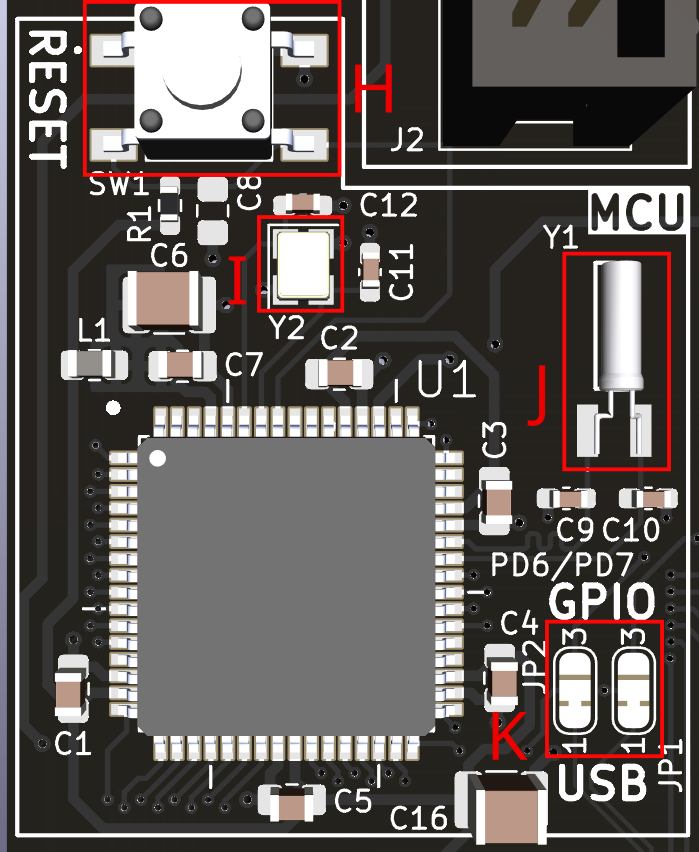
\includegraphics[width=10cm]{mcu.png}
			\caption{Sekcja mikrokontrolera}
			\label{mcu}
		\end{figure}
	\section{USB}
		Złącze micro USB może być wykorzystane również do przesyłu danych dzięki wbudowanemu interfejsowi USB mikrokontrolera. Interfejs USB jest współdzielony z niektórymi GPIO (patrz:schemat). Złącze K z rysunku \ref{mcu} służy do konfigurowania połączenia USB. Domyślnie do mikrokontrolera podłączona jest linia danych USB, a wyprowadzenia GPIO są odłączone. Istnieje możliwość odłączenia linii danych i podłączenia do wyprowadzeń GPIO. W tym celu należy przeciąć ścieżkę pomiędzy polami lutowniczymi 1 (USB) i 2 (środkowe), a następnie zmostkowanie cyną pól 2 i 3 (GPIO). Należy to zrobić w obydwu złączach.
	
	\chapter{Dodatek A: Schemat układu}
		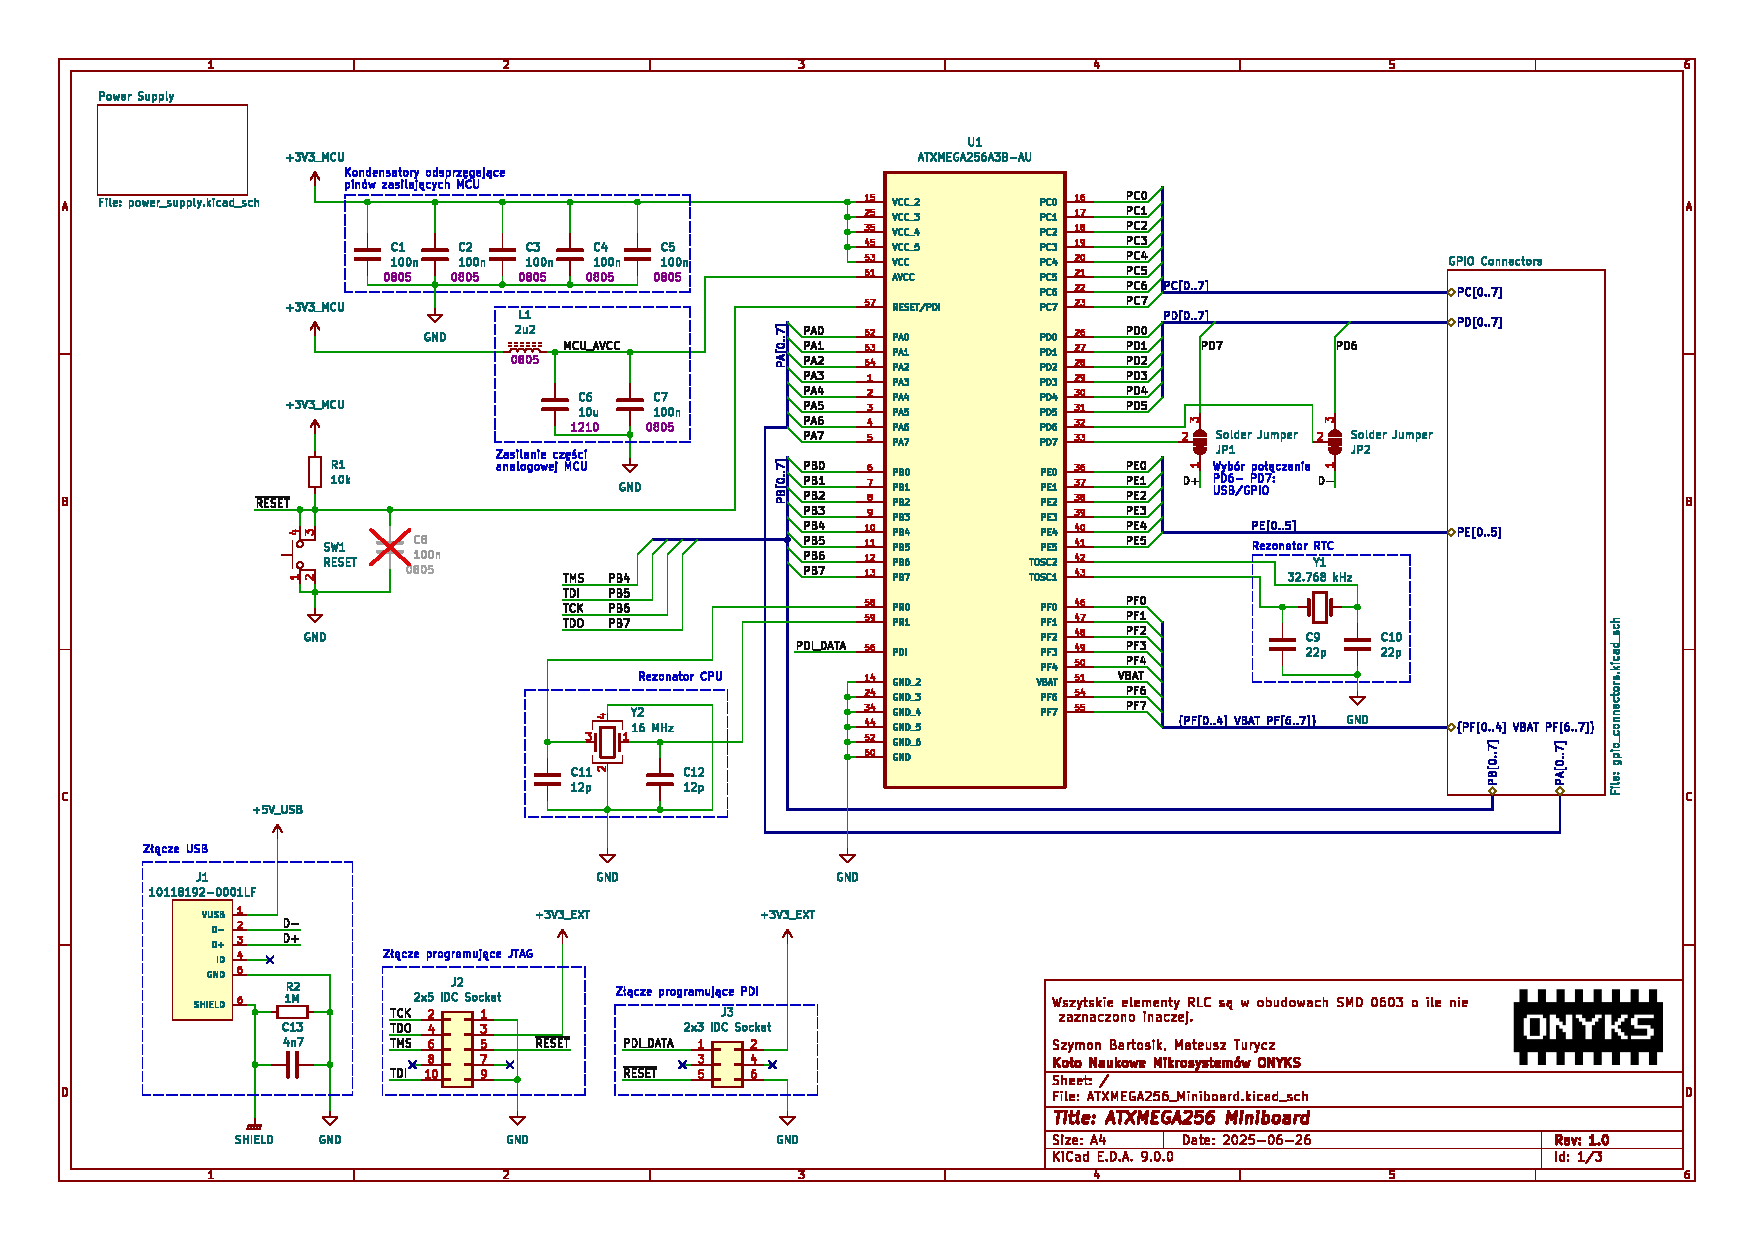
\includepdf[pages={-},angle=270]{../../schematics/ATXMEGA256_Miniboard.pdf}
	\chapter{Dodatek B: Schemat PCB}
		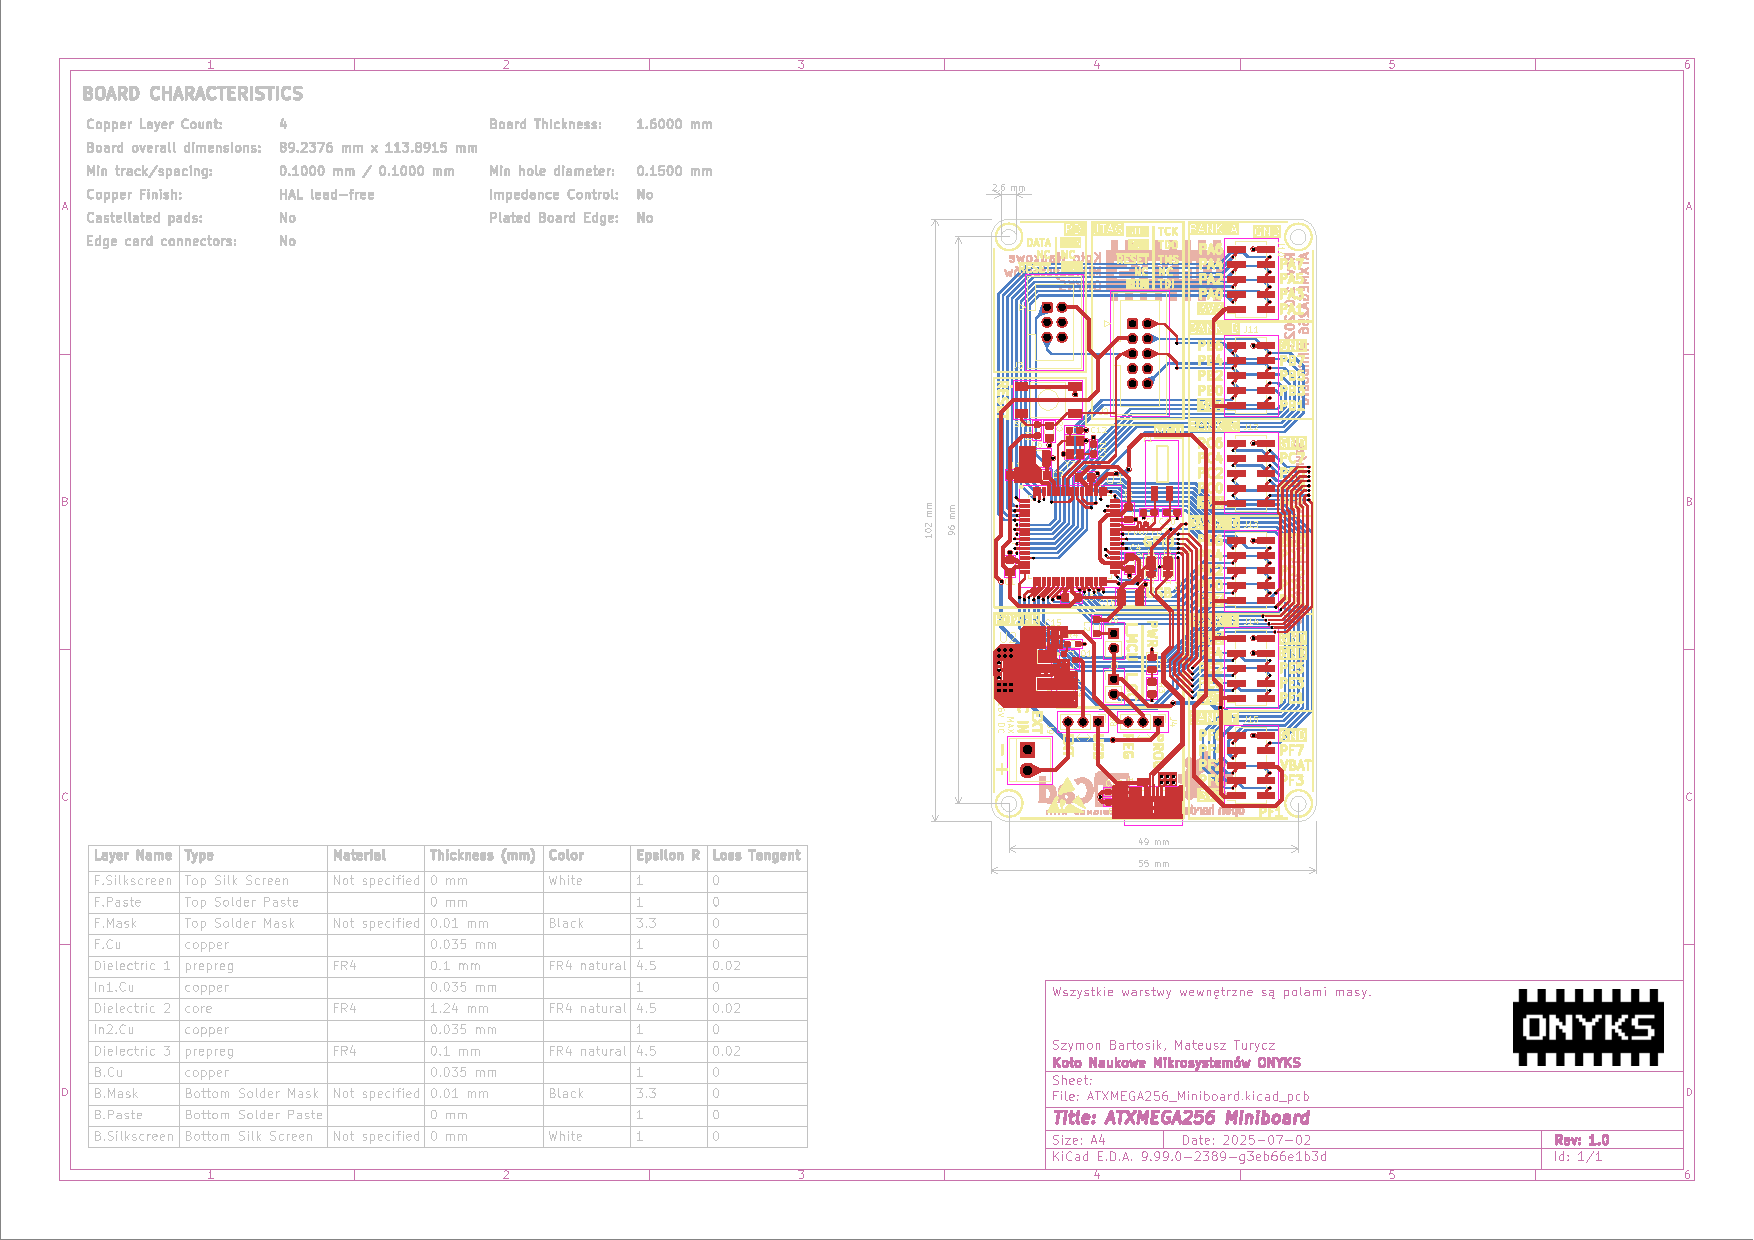
\includepdf[pages={-},angle=270]{../../pcb/ATXMEGA256_Miniboard_PCB.pdf}
\end{document}